% This file was created with tikzplotlib v0.9.16.
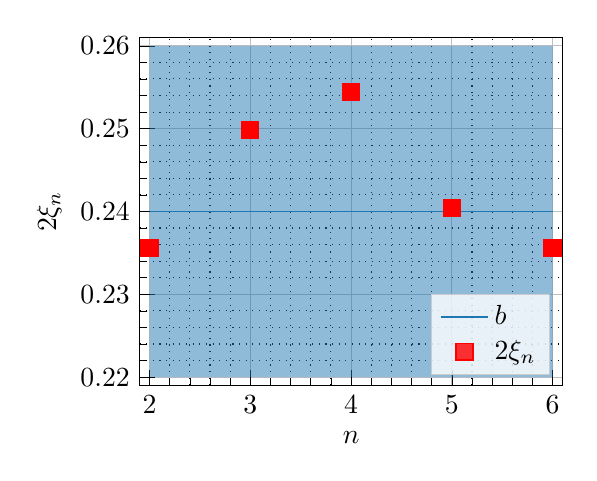
\begin{tikzpicture}

\definecolor{color0}{rgb}{0.12156862745098,0.466666666666667,0.705882352941177}

\begin{axis}[
legend cell align={left},
legend style={
  fill opacity=0.8,
  draw opacity=1,
  text opacity=1,
  at={(0.97,0.03)},
  anchor=south east,
  draw=white!80!black
},
height=6cm,
tick align=inside,
major tick length=0.2cm,
minor tick length=0.1cm,
tick pos=left,
xmin=1.9, xmax=6.1,
xtick={1, 2, 3, 4, 5, 6, 7},
minor x tick num=4,
xmajorgrids,
minor x grid style={dotted,black},
xminorgrids,
xtick style={color=black},
xlabel={$n$},
ymin=0.219, ymax=0.261,
ytick={0.21, 0.22, 0.23, 0.24, 0.25, 0.26, 0.27},
minor y tick num=4,
ymajorgrids,
minor y grid style={dotted,black},
yminorgrids,
ytick style={color=black},
ylabel={$2\xi_n$}
]
\path [fill=color0, fill opacity=0.5]
(axis cs:2,0.26)
--(axis cs:2,0.22)
--(axis cs:3,0.22)
--(axis cs:4,0.22)
--(axis cs:5,0.22)
--(axis cs:6,0.22)
--(axis cs:6,0.26)
--(axis cs:6,0.26)
--(axis cs:5,0.26)
--(axis cs:4,0.26)
--(axis cs:3,0.26)
--(axis cs:2,0.26)
--cycle;

\path [draw=red, semithick]
(axis cs:2,0.235281300991852)
--(axis cs:2,0.235836518666883);

\path [draw=red, semithick]
(axis cs:3,0.249455355580835)
--(axis cs:3,0.250240551946933);

\path [draw=red, semithick]
(axis cs:4,0.253918670617335)
--(axis cs:4,0.254946733983921);

\path [draw=red, semithick]
(axis cs:5,0.239736305603426)
--(axis cs:5,0.241096305603426);

\path [draw=red, semithick]
(axis cs:6,0.234726083316821)
--(axis cs:6,0.236391736341914);

\addplot [semithick, color0]
table {%
2 0.24
3 0.24
4 0.24
5 0.24
6 0.24
};
\addlegendentry{$b$}
\addplot [semithick, red, mark=square*, mark size=3, mark options={solid}, only marks]
table {%
2 0.235558909829367
3 0.249847953763884
4 0.254432702300628
5 0.240416305603426
6 0.235558909829367
};
\addlegendentry{$2\xi_n$}
\end{axis}

\end{tikzpicture}
